\subsection{Architecture du projet} \label{sec:architecture}

\subsubsection{Architecture système} \label{sec:architecture_système}
L'architecture du projet a été définie en fonction de contraintes matérielles, organisationnelles et structurelles strictes : capacité de calcul limitée du Raspberry Pi Zero, absence d'infrastructure réseau dédiée (pas de serveur central, de broker MQTT, ni de routeur intelligent), utilisation des robots dans le cadre d'autres recherches.  
Ces restrictions empêchent l’adoption de standards modernes de la robotique distribuée, comme l’utilisation du \acrfull{ros} ou du protocole \acrfull{mqtt}.

En réponse aux besoins exprimés dans les chapitres \ref{sec:specs} et \ref{sec:limites}, et en cohérence avec les conclusions du chapitre \ref{sec:conclusion_recherches}, l’architecture adoptée repose sur les principes suivants :

\begin{itemize}
    \item \textbf{Communication directe via WebSocket} : un canal de communication bidirectionnel est établi entre le poste de contrôle (client) et chaque robot via un WebSocket dédié. 
    Cela évite toute dépendance à un serveur tiers comme dans le modèle MQTT.
    
    \item \textbf{Architecture orientée message} : chaque robot transmet indépendamment ses informations (capteurs, erreurs, logs) et reçoit des instructions ciblées, suivant une logique inspirée du modèle \textit{publisher/subscriber}, mais sans infrastructure centralisée.
    
    \item \textbf{Interface multi-robot} : l’interface cliente gère plusieurs connexions simultanées, permettant à l’utilisateur de visualiser, éditer et envoyer des programmes vers un ou plusieurs robots de manière indépendante.
\end{itemize}

\begin{figure}[H]
    \centering
    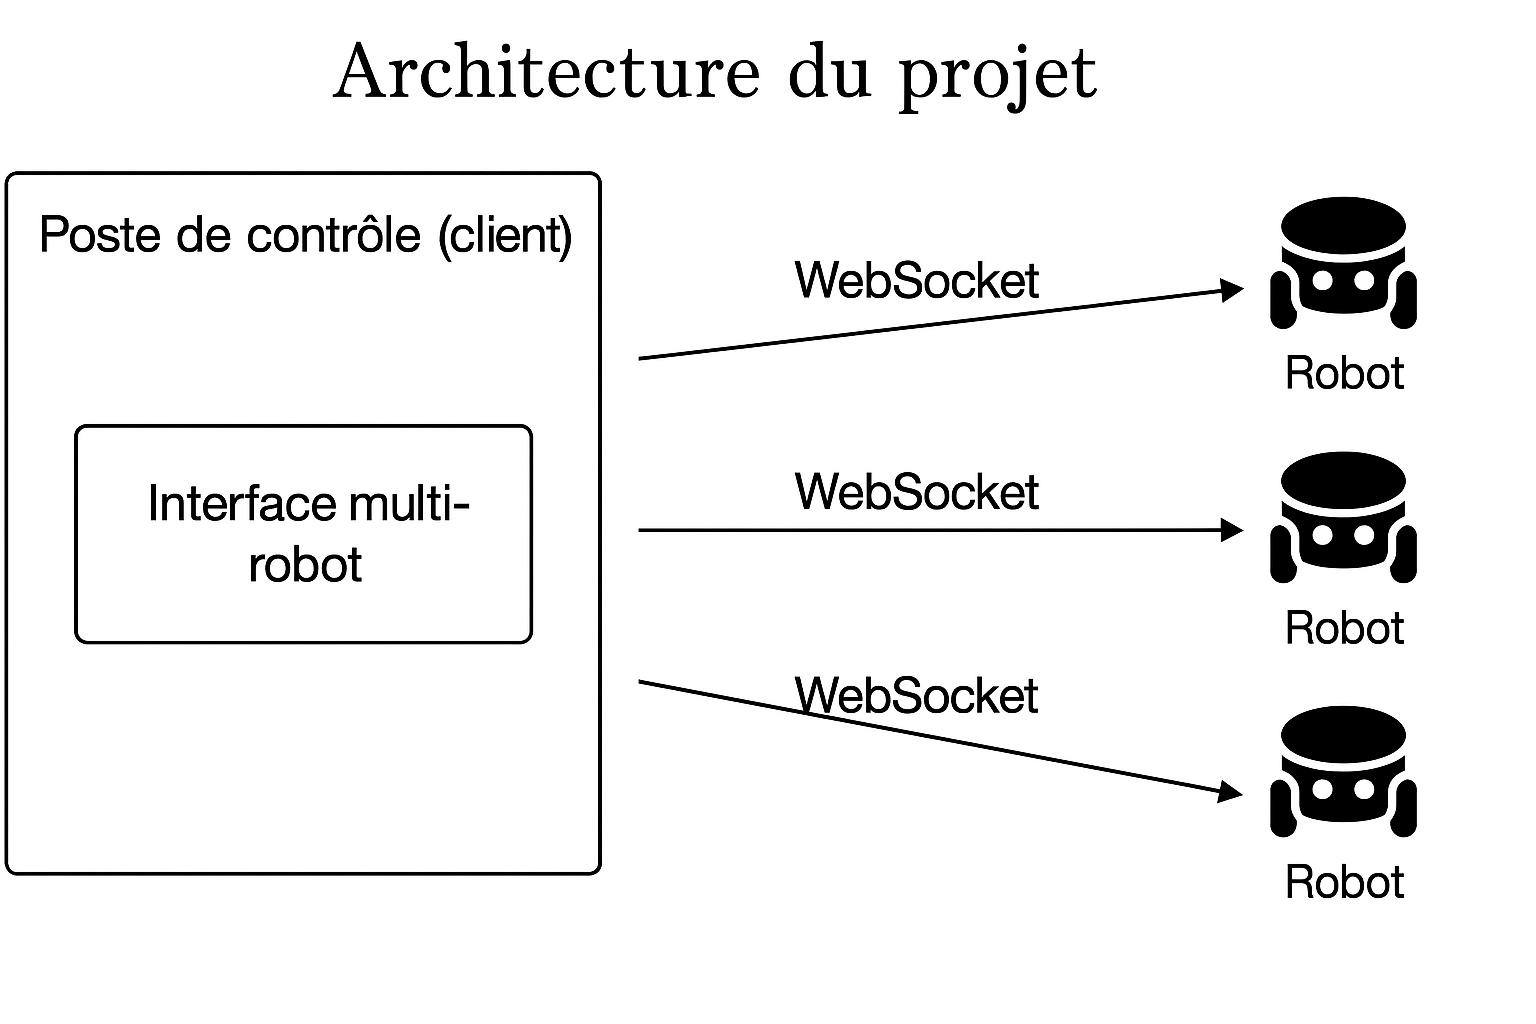
\includegraphics[width=0.8\linewidth]{.//figures//high_level_design.png}
    \caption{\label{fig:conceptual_hld} Schéma conceptuel de l'architecture logicielle du projet}
\end{figure}

Cette approche, bien qu’elle limite certaines options technologiques classiques, oriente l’architecture vers une solution à la fois légère, décentralisée (chaque robot se gère et communique avec le poste de contrôle) et facile à déployer.
Elle s’inspire des pratiques de la robotique moderne (comme \acrshort{ros}2) tout en les simplifiant pour rester cohérent avec les ressources limitées du robot.

\paragraph{Avantages et limites}
Le modèle retenu offre les mêmes avantages qu'un modèle distribué classique (tolérance aux pannes, modularité, déploiement simple, accessibilité).
Cependant, il présente également des limites importantes :
\begin{itemize}
    \item \textbf{Charge concentrée sur le poste de contrôle} : l’ordinateur client cumule plusieurs rôles (éditeur de code, gestionnaire de connexions, interface graphique, synchronisation), ce qui peut dégrader les performances si le matériel est peu puissant.
    
    \item \textbf{Pas d’état partagé} : l’absence de serveur central empêche toute coordination native entre les robots (pas de mémoire globale, pas de synchronisation multi-robot).
    
    \item \textbf{Pas de persistance des données} : les programmes, logs ou résultats ne sont pas sauvegardés automatiquement ; toutes les données peuvent être perdues en cas de crash.
    
    \item \textbf{Forte dépendance au réseau Wi-Fi} : toute perturbation du réseau peut compromettre l’expérience utilisateur.
\end{itemize}

Ces inconvénients ne remettent pas en cause la validité du modèle dans le cadre de ce projet, mais ouvrent des pistes d’amélioration pour une future version plus évoluée (voir \autoref{sec:axes_amelioration}).

\subsubsection{Architecture logicielle} \label{sec:architecture_logicielle}
Comme pour toute application bien conçue, l’objectif des standards de développement adoptés est de réduire le couplage entre les différents composants logiciels et les fonctionnalités qu’ils implémentent.

Dans le contexte spécifique de ce projet, qui vise à concevoir une interface de contrôle pour le robot e-puck2, un certain degré de couplage reste toutefois nécessaire, notamment au niveau des scripts de contrôle générés pour le robot.

Cela dit, la priorité reste de garantir une architecture logicielle assurant testabilité, maintenabilité et scalabilité. Si ces trois qualités peuvent être respectées à la fois dans le logiciel embarqué et dans l'interface utilisateur, on peut considérer que les objectifs de conception sont atteints.

Conformément aux réflexions menées dans un précédent travail de recherche, le choix s’est naturellement porté sur l’approche de la \textit{clean architecture} \autocite{tinael_devresse_analyse_2023}.
